\documentclass[runningheads]{llncs}

\usepackage[utf8]{inputenc}
\usepackage[T1]{fontenc}
\usepackage{graphicx}
\usepackage{float}
\usepackage{amsmath}
\usepackage{booktabs}
\usepackage{xcolor}
\usepackage{parskip}

\newcommand{\TODO}[1]{\textcolor{red}{\textbf{[TODO: #1]}}}

\begin{document}

\title{Evolving Super Mario Bros Controllers\\via Typed Genetic Programming}
\titlerunning{Evolving Mario Controllers via Typed GP}

% TODO: confirm group members
\author{Miguel Cabral Pinto \and Tiago Silva}
\authorrunning{M. Cabral Pinto and T. Silva}
\institute{Departamento de Engenharia Informática, Universidade de Coimbra\\
\email{\{mcp, tds\}@student.uc.pt}}

\maketitle

\begin{abstract}
We evolve game controllers for Super Mario Bros using Genetic Programming across three task variants: a Runner targeting level completion, a Hunter targeting enemy kills, and a Thief targeting coin collection. Each individual is a typed syntax tree that compiles to an executable Python function, so the search operates directly over the space of structured programs. We define a typed grammar giving agents access to a $22\times22$ grid of terrain and enemy data. Bloat is controlled through Double Tournament selection with parsimony pressure; generalization is promoted through a rotating seed pool that changes every 10 generations. \TODO{2 sentences: win rate achieved by the evolved agent, improvement over the random baseline.}
\end{abstract}


% =============================================================================
\section{Introduction}
% =============================================================================

% Platform games are a natural testbed for game AI: the state space is high-dimensional, level geometry varies across seeds, and success requires coordinating simple actions (jumping, running, stopping) into extended behavioral sequences, which rules out approaches that rely on differentiable objectives or explicit model access. The Mario AI framework~\cite{togelius2009mario} provides a reproducible instance of this setting, with a configurable difficulty axis and a socket-based API that allows external agents to control Mario at each simulation step.

In this work we use Genetic Programming (GP)~\cite{koza1992genetic} to evolve controllers for the Mario AI framework~\cite{togelius2009mario}. GP is well-matched to this problem for two reasons: it requires only a scalar fitness signal and no gradient information, and it produces programs as output, meaning the evolved controller is a readable Python function. Since the failure mode of any agent is visible in the code, iterating on the fitness function is fast and targeted.

The course provided a base GP repository implemented with DEAP~\cite{fortin2012deap}: a minimal random search over a small typed grammar with two senses (\texttt{on\_ground}, \texttt{can\_jump}), two actions (\texttt{RIGHT}, \texttt{JUMP}), and basic \texttt{IF}/\texttt{SEQ} program structure. During our work, we expanded the grammar to give agents better perception of terrain and enemies, designed the fitness function, and replaced the random search with a full evolutionary algorithm.

Three task variants were evaluated: a Runner task targeting level completion, a Hunter task rewarding enemy kills, and a Thief task rewarding coin collection. The fitness function went through several iterations; the choices behind the final version are described in Section~\ref{sec:fitness}.


% % =============================================================================
% \section{Background}
% \label{sec:background}
% % =============================================================================

% Evolutionary Algorithms (EAs)~\cite{back1996evolutionary} search by maintaining a population of candidate solutions and iteratively improving it through selection and variation. Selection identifies fitter individuals as parents; crossover recombines their genetic material to produce offspring; mutation introduces random perturbations to maintain diversity. Since EAs require only a scalar fitness score and impose no smoothness assumptions on the objective, they are a natural fit for black-box simulators such as the Mario framework, where no gradient of the fitness function is available.

% Genetic Programming~\cite{koza1992genetic} applies this scheme to programs. Individuals are syntax trees in which internal nodes are functions drawn from a \emph{function set} and leaves are constants or input variables from a \emph{terminal set}. The key practical challenge is \emph{bloat}: programs tend to grow in size over generations without corresponding fitness improvement, since non-contributing code segments are protected from disruption by genetic operators and gradually accumulate~\cite{luke2006bloat}. Unchecked bloat slows evaluation, reduces interpretability, and eventually saturates memory. We address it through the selection scheme described in Section~\ref{sec:ea}.

% Typed GP~\cite{montana1995strongly} attaches explicit input and return types to each primitive, so the grammar defines typed production rules and every tree the system can generate is type-consistent by construction. In the context of evolving executable code, this means every individual compiles without error, which eliminates a common source of wasted evaluations in untyped GP formulations.


% =============================================================================
\section{Methodology}
\label{sec:method}
% =============================================================================

\subsection{Environment}
\label{sec:env}

The Mario AI framework~\cite{togelius2009mario} is a Java simulator that exposes a socket API through which external agents send action vectors and receive observations at a fixed step rate. At each step the agent receives information about the simulation (e.g., Mario state \& position, level scene observation grid).

The agent outputs a boolean vector $[\texttt{LEFT},\,\texttt{RIGHT},\,\texttt{DOWN},\,\texttt{JUMP},\,\texttt{SPEED}]$ at each step, controlling Mario's actions. Difficulty is controlled along two independent axes: mario mode (small, large, or fire) and level difficulty, which scales obstacle density and enemy variety.

\subsection{Typed Grammar and Representation}
\label{sec:grammar}

Each individual is a program tree in a typed grammar built on top of the provided DEAP~\cite{fortin2012deap} scaffold. We extended the original four types (\texttt{Cond}, \texttt{Key}, \texttt{Bool}, \texttt{Expr}) to nine: \texttt{Program}, \texttt{Stmt}, \texttt{Cond}, \texttt{Comparator}, \texttt{Key}, \texttt{Bool}, \texttt{Offset}, \texttt{EnemyKind}, and \texttt{TileValue}.

\paragraph{Program structure.}
A \texttt{Program} is a non-empty sequence of statements built left-recursively:
\[
\text{Program} \to \texttt{END}(\text{Stmt}) \mid \texttt{SEQ}(\text{Stmt},\,\text{Program})
\]

\paragraph{Statements.}
A \texttt{Stmt} is a conditional branch or a direct key assignment:
\[
\text{Stmt} \to \texttt{IF}(\text{Cond},\,\text{Stmt}) \mid \texttt{IF\_ELSE}(\text{Cond},\,\text{Stmt},\,\text{Stmt}) \mid \texttt{SET\_ACTION}(\text{Key},\,\text{Bool})
\]

\paragraph{Conditions.}
Conditions combine two perception predicates with standard boolean connectives:
\begin{align*}
\text{Cond} \to{}& \texttt{AND}(\text{Cond},\text{Cond}) \mid \texttt{OR}(\text{Cond},\text{Cond}) \mid \texttt{NOT}(\text{Cond}) \\
  \mid{}& \texttt{CheckEnemyAt}(\text{Offset}_x,\,\text{Offset}_y,\,\text{Comparator},\,\text{EnemyKind}) \\
  \mid{}& \texttt{CheckLandscapeAt}(\text{Offset}_x,\,\text{Offset}_y,\,\text{Comparator},\,\text{TileValue}) \\
  \mid{}& \texttt{IsMarioOnGround} \mid \texttt{MayMarioJump}
\end{align*}

Both predicates access the $22\times22$ grid at offset $(\Delta x, \Delta y)$ relative to Mario's cell. Horizontal offsets $\Delta x \in \{0,1,2,3\}$ let the agent look ahead up to four cells; vertical offsets $\Delta y \in \{-3,\ldots,+3\}$ cover above and below. The rationale behind this is that giving it full grid visibility would lead an explosion of possible programs, while this small subset allows for sufficient behavioral coverage while allowing it to learn to react to close threats. Additionally, since the framework stores terrain and enemy data in the same grid, both predicates query the same array and differ only in the value range they compare against: enemy type codes ($2$--$13$) versus tile codes.

An earlier version of the grammar used precomputed boolean predicates computed outside the GP tree (\texttt{hole\_ahead}, \texttt{enemy\_ahead}, \texttt{wall\_ahead}). This simplified the search space but also reduced it: the agent could not, for example, distinguish between enemy types or check arbitrary offsets. Though experiments with this grammar offered interesting insights (discussed below), these changes were reverted in order to align with the project statement's scope.

\paragraph{Terminals.}
Enemy kind terminals cover all sprite types: Goomba (standard and winged), Red and Green Koopa (standard and winged), Bullet Bill, Spiky (standard and winged), Piranha Flower, and Shell. Tile value terminals are \textsc{HardObstacle} ($-10$), \textsc{Brick} ($16$), and \textsc{EnemyObstacle} ($20$). Action key terminals are \textsc{Right}, \textsc{Left}, \textsc{Jump}, \textsc{Speed}, and \textsc{Down}.

% \paragraph{Initialization.}
% The provided scaffold includes a \emph{safe grow} initialization procedure that enforces type constraints and targets depths between $3$ and $6$, checking type feasibility before selecting any primitive. DEAP's standard grow method produces degenerate trees near type boundaries in strongly-typed grammars, since it does not account for mandatory argument chains; the safe grow procedure avoids these dead ends and was kept unchanged.

\subsection{Fitness Calculation}
\label{sec:fitness}

Three task variants were implemented: Runner, Hunter, and Thief. All three use the same per-step reward function; the difference is the episode-level bonus each adds to target its secondary objective.

\subsubsection{Common Reward}

Every task uses the following per-step reward:

\begin{equation}
r_t = \Delta x_t + P_{\text{stuck}}(t)
\label{eq:step_reward}
\end{equation}

\paragraph{Forward progress.}
$\Delta x_t = \mathbf{1}[\,x_t - x_{t-1} \geq 0.61\,]$ awards one point when Mario advances at least $0.61$ world units in a step. The binary form means walking and running at full speed score identically, since faster movement does not inherently produce better behavior given the grammar's limited action space. The threshold also prevents stationary oscillations near a wall from accumulating reward, which would work against the stuck penalty.

\paragraph{Stuck penalty.}
When Mario has made no forward progress for more than $10$ consecutive steps and a solid obstacle occupies the cell directly ahead, a growing penalty is applied:
\begin{equation}
P_{\text{stuck}}(t) = \begin{cases}
    -10\,(n_{\text{stuck}} - 10) & \text{if } n_{\text{stuck}} > 10 \text{ and obstacle ahead} \\
    0 & \text{otherwise}
\end{cases}
\end{equation}
The 10-step grace period prevents the penalty from firing during legitimate pauses. The condition also requires that no Piranha Flower is present in the column above Mario, given that the original formulation without this check caused agents to rush into Piranha pipes instead of waiting for the enemy to retract.

\paragraph{Airtime penalty.}
A behavior that emerged early in training was a tendency to jump constantly. Given the grammar's limited expressive power, evolving a principled jump strategy is difficult; jumping on every possible frame clears a large fraction of obstacles and pits, which makes it a highly fit strategy in early generations. Once a population converges on it, there is no selection pressure toward a more targeted approach.

To counteract this, we tested a penalty proportional to total airtime across several iterations. The results were binary: either the penalty was too weak to suppress the behavior, or strong enough to also prevent agents from learning to jump at all, blocking forward progress entirely. This pointed to the conclusion that the current grammar does not provide enough perceptual structure for agents to learn when jumping is warranted. Additionally, agents evolved before removing the initial complex perceptions from our grammar (e.g., \texttt{hole\_ahead}) did not exhibit constant jumping, which further supports this interpretation.

\subsubsection{Runner Task}

The Runner task targets level completion. Beyond the progress reward, a win bonus of $W = 10{,}000$ is added at the end of any episode in which Mario clears the level:

\begin{equation}
B_{\text{runner}}(s,d) = W \cdot \mathbf{1}[\text{win}_{s,d}], \quad W = 10{,}000
\end{equation}

\subsubsection{Hunter Task}

The Hunter task targets enemy kills. The episode bonus is proportional to the number of confirmed kills $\hat{K}_{s,d}$ accrued during the episode:

\begin{equation}
B_{\text{hunter}}(s,d) = K \cdot \hat{K}_{s,d}, \quad K = 10{,}000
\end{equation}

Kill detection compares the enemy list between consecutive frames, counting reductions in enemy count while handling the exceptions that occur with enemies from the first three difficulties: Koopa-to-Shell transitions (a Koopa count drop paired with a Shell count rise maintains the enemy list size, but is counted as a kill); enemies falling into pits (filtered by a $y$ position threshold); enemies scrolling off-screen as Mario advances (filtered by horizontal distance); and Piranha Flowers retracting into pipes (detected by tracking per-column disappearances). A disappearing enemy is counted as a kill only if Mario's vertical velocity at that step is consistent with a stomp bounce, meaning a sign reversal or deceleration pattern matching a rebound off the top of an enemy.

This replaced an earlier heuristic that counted kills whenever the number of enemies within a small radius around Mario decreased between frames. That approach produced frequent false positives in crowded sections, inflating the reward signal and leading agents to stand still near enemy clusters rather than completing the level.

An earlier design combined kills and coin collection into a single secondary objective. Optimizing for both goals simultaneously, with the limited grammar available to agents, added the workload of testing different weight configurations, and early experiments resulted in suboptimal agent performances across both tasks. Therefore, we created the Thief agent, splitting kills and coins into separate tasks, allowing each population to specialize on one behavior.

\subsubsection{Thief Task}

The Thief task targets coin collection. Coin counts are read directly from the end-of-episode observation packet provided by the game framework, so no per-step detection is needed. The episode bonus is:

\begin{equation}
B_{\text{thief}}(s,d) = C \cdot \hat{N}_{s,d}, \quad C = 2{,}500
\end{equation}

where $\hat{N}_{s,d}$ is the total coins collected in the episode. The per-coin bonus ($2{,}500$) is set lower than the kill bonus ($10{,}000$) given that coins are more abundant than killable enemies in a typical level; a higher value would have dominated the forward-progress signal and incentivized agents to loop back and re-collect rather than advance.

\subsubsection{Episode Fitness}

Each individual is evaluated over a seed pool $\mathcal{S}$ of $5$ level seeds and $3$ consecutive difficulty levels starting at base difficulty $d_{\text{base}}$. Fitness is the mean total reward across all $|\mathcal{S}| \times 3$ episodes:

\begin{equation}
F = \frac{1}{|\mathcal{S}|} \sum_{s \in \mathcal{S}} \sum_{d=d_{\text{base}}}^{d_{\text{base}}+2} \!\Bigl(\sum_t r_t + B_{\text{task}}(s, d)\Bigr)
\label{eq:fitness}
\end{equation}

where $B_{\text{task}}(s, d)$ is the task-specific episode bonus defined below.

\subsection{Evolutionary Algorithm}
\label{sec:ea}

Table~\ref{tab:params} lists the final parameter configuration.

\begin{table}[t]
\caption{Evolutionary algorithm parameters used in the main experiments.}
\label{tab:params}
\centering
\begin{tabular}{ll}
\toprule
\textbf{Parameter} & \textbf{Value} \\
\midrule
Population size & 100 \\
Generations & 300 \\
Crossover rate ($p_c$) & 0.6 \\
Mutation rate ($p_m$) & $1.0 \to 0.4$ (linear over training) \\
Crossover operator & One-point (\texttt{gp.cxOnePoint}) \\
Mutation operator & Uniform subtree (\texttt{gp.mutUniform}) \\
Selection & Double Tournament \\
\quad Fitness tournament size & $2 \to 7$ (linear over training) \\
\quad Parsimony tournament size & 1.7 \\
Max tree height & 10 \\
Elitism & Top-1 (Hall of Fame) \\
\bottomrule
\end{tabular}
\end{table}

\paragraph{Selection and bloat control.}
We use Double Tournament selection~\cite{luke2006bloat}, which runs two nested tournaments: the outer selects based on fitness (with a size that grows from 2 to 7 over training), and the inner selects based on tree size with a fractional tournament of size $1.7$, preferring shorter programs when fitness is similar. This avoids adding a size term to the fitness function directly, which requires careful weighting.

\paragraph{Crossover and mutation.}
One-point crossover selects a random node in each parent and swaps the corresponding subtrees. If the resulting offspring exceeds height $10$, the operation is reverted and the parent is preserved. Uniform subtree mutation selects a random node and replaces its subtree with a freshly grown random subtree (depth 2 - 6), so the algorithm introduces genuinely new code fragments rather than only recombining existing material.

The mutation rate decreases from $1.0$ to $0.4$ over training. Preliminary experiments with fixed rates struggled with keeping an appropriate balance between exploration and exploitation at different points in the experiment. The dynamic schedule addresses this: high mutation early for exploration, lower mutation late for exploitation. The rationale behind the fitness tournament size is the same: it grows linearly so that early generations explore broadly under low selection pressure and later generations converge under stronger pressure once the search has found promising regions.

\paragraph{Elitism.}
The single best individual across all generations, stored in a Hall of Fame, is copied directly into the next generation at each step. This ensures the best fitness found is never lost to a bad crossover or mutation.

\paragraph{Parallelism.}
The provided evaluation infrastructure distributes fitness evaluations across $5$ worker processes, each holding a persistent connection to its own simulator instance. We extended it to support multi-seed pools, difficulty scheduling, and lazy re-evaluation: given the simulation's deterministic nature, only individuals whose fitness was invalidated need to be re-evaluated.


% =============================================================================
\section{Experimental Design}
\label{sec:exp}
% =============================================================================

\subsection{Evaluation Protocol}

All individuals within a generation are evaluated on the same $5$ randomly drawn level seeds, so that fitness values are directly comparable within a generation. Using different seeds per individual, as we did in early experiments, introduced noise that made selection unreliable: an individual with higher fitness might simply have faced an easier level rather than exhibiting a better strategy, which led to the population stagnating on a few lucky seeds rather than improving.

To prevent overfitting to specific levels, the seed pool is rotated every $10$ generations by drawing a fresh set from a universe of $1{,}000$ seeds. At each rotation, all population fitnesses are invalidated and re-evaluated under the new pool, including the Hall of Fame champion (so its score always reflects the current pool). A checkpoint is saved at each rotation. At the end of training, all checkpoints are re-evaluated on a fixed set of $500$ held-out seeds across the three training difficulties. The Hall of Fame champion from the checkpoint with the highest overall win rate on this held-out set is selected as the final evolved agent. This re-evaluation step is necessary because the Hall of Fame score stored in each checkpoint reflects fitness under whichever seed pool was active during that rotation, making raw fitness values across checkpoints incomparable without a shared evaluation basis. This method also allows for the visualization of performance across generations, as seen in Figure \ref{fig:normal_100}.

\begin{figure}[h]
  \centering
  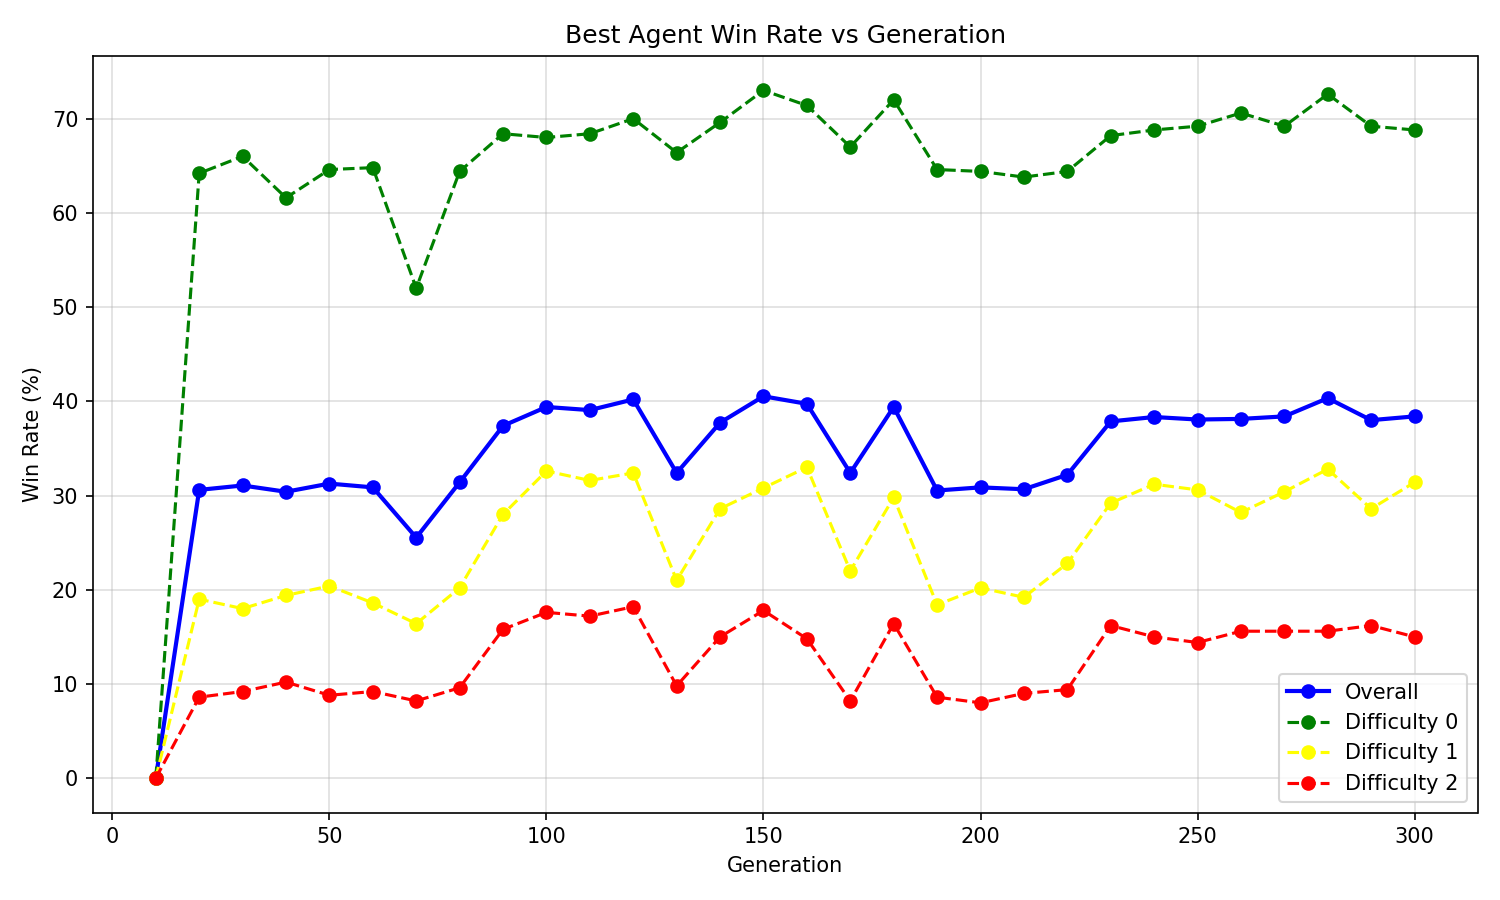
\includegraphics[width=0.82\textwidth]{images/winrate_vs_gen_normal_100.png}
  \caption{Example champion win rate vs.\ generation plot for the Runner task. After reaching finding a capable strategy (running and jumping), it hovers around 30-40\% win-rate, attempting to optimize its strategy until the end of the training run. Completion rate per level closely follows the swings in the overall rate.}
  \label{fig:normal_100}
\end{figure}

For seed pool rotation, periods of 5, 10, and 20 generations were compared, with the middle option achieving overall better results. Rotating every 5 generations did not give the population enough time to exploit each seed pool before it changed, slowing convergence. Rotating every 20 generations allowed the population to overfit to specific level seeds, with agents that scored well on the current pool but failed to generalize when the pool changed. Rotating every 10 generations provided a good balance: enough stability for selection to act meaningfully, and enough change to prevent overfitting.

The base difficulty $d_{\text{base}}$ is fixed at $0$ throughout training, so agents are always evaluated on difficulties $0$, $1$, and $2$ simultaneously. An earlier design explored a curriculum that gradually shifted $d_{\text{base}}$ upward over generations. This was abandoned when training on all three difficulties from the start produced better-generalizing agents, likely because the easier difficulty levels provide a reliable learning signal even when the population is still immature.

Finally, we chose to run 300-generation runs as a compromise between computational cost and exploration of the evolutionary approach. 200-individual and 100-individual populations were compared, with the latter configuration producing comparable completion rates at half the cost, and was adopted as the default.

\subsection{Comparative Baseline}

Evolved champions are compared against a random search baseline to separate the contribution of the evolutionary process from the expressive power of the grammar alone. We run five independent experiments per task variant, each with a different random seed. For each run, the champion is selected by re-evaluating all checkpoints on a shared held-out set, using win rate as the selection criterion for Runner, average kills for Hunter, and average coins for Thief. The baseline for each run is a single program drawn uniformly at random from the same grammar, with no selection or recombination applied. Both agents are then evaluated on $5{,}000$ held-out level seeds across three difficulty levels ($15{,}000$ episodes per agent per run), and we report mean and standard deviation across the five runs.

% As a further comparison, we replicated the full experiment with Mario initialized as \textit{big Mario} carrying a fire flower (hereafter \textit{Fire Mario}). The grammar was extended with a \texttt{fire} action, but all training and evaluation parameters (population size, generations, seed pool rotation, checkpoint selection, and held-out set size) remained identical. Descriptive statistics for Fire Mario are presented together with the normal Mario results in Table~\ref{tab:results}. Formal significance testing was reserved for the primary comparison.

\subsection{Statistical Analysis}

The evolutionary process and level generator are both stochastic, so a single run per task is not sufficient to draw reliable conclusions~\cite{doe_lecture}. Across the five independent runs per variant, we report mean and standard deviation for completion rate, average distance in unbeaten levels, enemies killed, and coins collected: mean number of coins gathered per episode. To quantify the advantage over the random baseline, we conducted paired-sample $t$-tests on the relevant metrics for each task variant.


% =============================================================================
\section{Results and Analysis}
\label{sec:results}
% =============================================================================

Table~\ref{tab:comparison} compares evolved champions against the random search baseline across all three task variants, evaluated on $5{,}000$ held-out seeds $\times$ 3 difficulties:

\begin{table}[H]
\caption{Evolved champions vs.\ random search baseline across task variants ($5{,}000$ seeds $\times$ 3 difficulties, mean $\pm$ std across 5 runs). \TODO{Fill in all values.}}
\label{tab:comparison}
\centering
\begin{tabular}{lcccc}
\toprule
\textbf{Metric} & \textbf{Random Baseline} & \textbf{Runner} & \textbf{Hunter} & \textbf{Thief} \\
 & \textbf{(Avg $\pm$ Std)} & \textbf{(Avg $\pm$ Std)} & \textbf{(Avg $\pm$ Std)} & \textbf{(Avg $\pm$ Std)} \\
\midrule
Levels Cleared (\%) & \TODO{X} & \TODO{Y} & \TODO{Y} & \TODO{Y} \\
Max Distance (px)   & \TODO{X} & \TODO{Y} & \TODO{Y} & \TODO{Y} \\
Enemies Killed      & ---      & ---      & \TODO{Y} & ---      \\
Coins Collected     & ---      & ---      & ---      & \TODO{Y} \\
\bottomrule
\end{tabular}
\end{table}

\TODO{Comment on the table. Describe the qualitative difference in behavior: the random agent will jump and move without a coordinated strategy, while the evolved agent should show consistent forward movement and at minimum a learned response to walls and pits. Discuss whether the improvement is meaningful given the observed standard deviations, or whether the variance is too large to draw firm conclusions.}

% \subsection{Qualitative Analysis of Evolved Behavior}

% The best individual found in the 100-population normal-mode run (Hall of Fame score: 51114) is shown below.

% \begin{small}
% \begin{verbatim}
% def corre(action, landscape, enemies, can_jump,
%           on_ground, mario_pos, Mario, Sprite, **kwargs):

%     if (enemies[11+-1][11+1] < 8):
%         if (not (landscape[11+1][11+3] > 16)):
%             if (enemies[11+-1][11+1] < 12):
%                 if (not (on_ground or on_ground)):
%                     action[Mario.KEY_RIGHT] = 1
%                 else:
%                     action[Mario.KEY_SPEED] = 1
%         else:
%             action[Mario.KEY_SPEED] = 1
%     if ((not (on_ground or ((enemies[11+0][11+2] < 13)
%          and ((enemies[11+0][11+-3] == 13) or on_ground))))
%          or can_jump):
%         action[Mario.KEY_JUMP] = 1
%     else:
%         if (landscape[11+0][11+3] < 16):
%             if (not (enemies[11+-2][11+0] == 8)):
%                 if can_jump:
%                     if (enemies[11+3][11+0] == 8):
%                         if can_jump:
%                             action[Mario.KEY_SPEED] = 0
%                         else:
%                             if on_ground:
%                                 action[Mario.KEY_LEFT] = 1
%                     else:
%                         if (can_jump and on_ground):
%                             if on_ground:
%                                 action[Mario.KEY_RIGHT] = 1
%                         else:
%                             if can_jump:
%                                 action[Mario.KEY_LEFT] = 1
%                             else:
%                                 action[Mario.KEY_RIGHT] = 1
%             else:
%                 if can_jump:
%                     if (enemies[11+3][11+3] < 8):
%                         if can_jump:
%                             if can_jump:
%                                 action[Mario.KEY_DOWN] = 0
%                             else:
%                                 action[Mario.KEY_LEFT] = 0
%         else:
%             if can_jump:
%                 action[Mario.KEY_JUMP] = 0
% \end{verbatim}
% \end{small}

% The program consists of two sequential statements. The first block handles the speed decision: it checks for an enemy of type $< 8$ (Goomba or empty) one cell above and one cell ahead, and, if no tile with code $> 16$ (i.e., no enemy obstacle) blocks the path three columns ahead at ground level, sets \textsc{Speed}. This increases forward momentum whenever a low-threat enemy is nearby and the terrain ahead is passable.

% The second block encodes the dominant behavior. Its condition, \texttt{(not (on\_ground or \ldots)) or can\_jump}, simplifies to \texttt{can\_jump} on almost every ground-contact frame, meaning the agent jumps on every step it is able to. The result is a controller that runs right and jumps continuously, with the speed modulation in the first block providing the only enemy-sensitive adjustment.

% The tree contains several introns. \texttt{on\_ground or on\_ground} evaluates identically to \texttt{on\_ground} but occupies two leaf nodes and one OR node. The else branch of the jump condition (lines 18--44) covers the brief window when Mario is grounded but \texttt{can\_jump} is false; since this window lasts only a few frames per landing, most of the nested conditions in that branch are rarely reached during a normal episode. Parsimony pressure kept the tree from growing further but did not eliminate these segments, since their size contribution was small enough to survive the parsimony tournament.

% The agent's primary failure mode is the absence of spatial lookahead in the jump decision: the jump fires based on \texttt{can\_jump} alone, without checking whether a pit or an obstacle lies ahead. On higher-difficulty levels with more pits and denser enemy placement, this causes the agent to launch itself into gaps it could have avoided, which accounts for the sharp drop in win rate from difficulty~0 to difficulty~2.


% =============================================================================
\section{Conclusion}
\label{sec:conclusion}
% =============================================================================

\TODO{Write after results are confirmed. Structure: (1) one paragraph restating the approach and the two objectives. (2) The most impactful design choices, with results woven in, e.g., ``Switching to the type-aware kill detector raised confirmed kills per episode from X to Y; the radius heuristic had attributed those same kills to off-screen scrolling.'' (3) Limitations: fixed-arity grammar with no loops or arithmetic, evaluation cost constraining population size, sensitivity to kill-reward weighting relative to the progress signal. (4) Future directions: extending the grammar with loops and numeric comparisons, island models to maintain diversity across subpopulations, and adaptive operator tuning via CMA-ES.}


\bibliographystyle{splncs04}
\bibliography{references}

\end{document}


%%% ============================================================
%%%  REPORT TODO LIST
%%% ============================================================
%%%
%%%  BLOCKING (need data before writing):
%%%  [ ] Abstract: 2 sentences with key results (win rate / kills / coins, improvement over random).
%%%  [x] Sec 5.1: convergence discussion written from the three plot images.
%%%  [ ] Table 2: fill all cells (Levels Cleared %, Max Distance, Enemies Killed, Coins Collected)
%%%      for Random Baseline, Runner, Hunter, and Thief columns.
%%%      Run evaluate_best_agent.py (5000 seeds × 3 difficulties) for each task variant
%%%      and a comparable random baseline.
%%%  [ ] Sec 5.2 comments: qualitative difference in behavior per task; significance given std.
%%%  [x] Sec 5.3: best individual pasted and analyzed (gp_mario_best.py).
%%%  [ ] Sec 6 (Conclusion): write after Table 2 is filled.
%%%
%%%  CLARIFICATIONS (resolved):
%%%  [x] --difficulty-shift: fixed at 0 throughout. Curriculum shift was explored
%%%      and abandoned; training on all 3 difficulties simultaneously from the
%%%      start produced better generalization. Now in the text.
%%%  [x] Seed rotation: 10 > 5 (too noisy) and 10 > 20 (overfitting). Now in text.
%%%  [x] Mario mode: default 0 (small Mario) in all main experiments.
%%%  [x] Champion evaluation: 5000 seeds × 3 difficulties per agent. Confirmed.
%%%  [x] Statistical evaluation: 5 independent full runs per task variant.
%%%  [x] Hunter/Thief split: single combined secondary objective caused poor performance
%%%      on both goals; separated into distinct tasks (Hunter=kills, Thief=coins).
%%%  [x] Champion selection: Runner → max win rate; Hunter → max avg kills; Thief → max avg coins.
%%%
%%%  STILL OPEN:
%%%  [ ] Fire-mode figure (Fig. 3) used 200-pop — treat as secondary / leave for
%%%      later. If comparing pop sizes, do it in its own ablation entry; otherwise
%%%      just present 100-pop as the main setting and note fire mode separately.
%%%  [ ] Hunter/Thief convergence plots — analogous to Figs 1–3 for kills and coins.
%%%
%%%  POLISH (low priority, do last):
%%%  [ ] Add axis labels to all 3 figures.
%%%  [ ] Revise intro final paragraph once results are in.
%%%  [ ] Verify author emails in \institute.
%%%  [ ] Optional: add a figure showing the compiled code of the best individual.
%%% ============================================================

% make it so that references appear in the order they are referenced
% see if all references are truly necessary
% mention fire mario as a note below actual results